\section{Results}

\begin{figure*}[t]
\centering
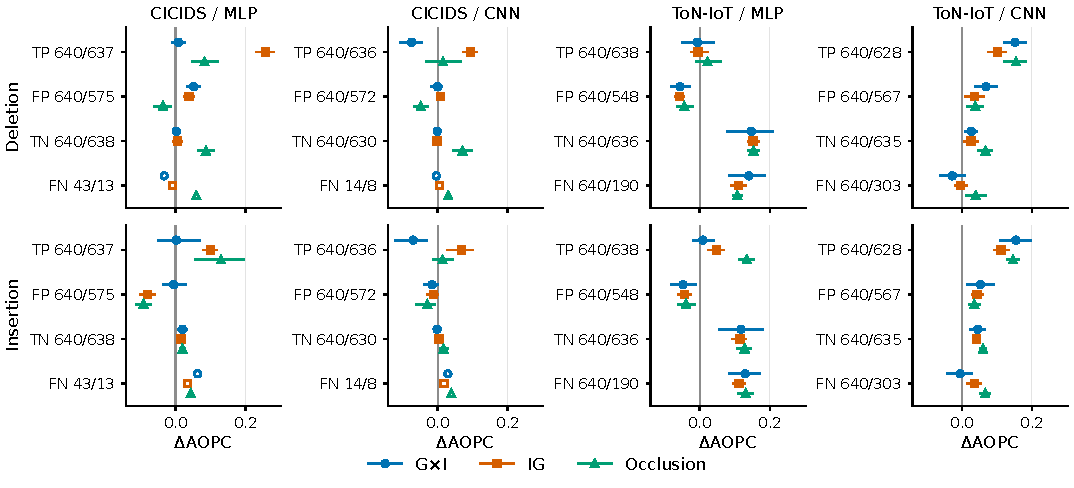
\includegraphics[width=\textwidth]{assets/binary_outcomes.pdf}
\caption{RQ3: training-median functional response on model-specific outcome
panels, separately for deletion and insertion. Labels give source--seed
records/distinct sources; methods within a condition share them. Bars show
marginal 95\% source/seed intervals. Open points without bars denote
low-support CICIDS false negatives, retained only descriptively. Targets
are attack for TP/FP and benign for TN/FN. No averaging across methods,
architectures or outcome strata is used.}
\label{fig:outcomes}
\end{figure*}

\subsection{Predictive Context}

Across five seeds, mean test F1 is .9798 (MLP) and .9821 (CNN) on CICIDS,
and .9740/.9728 on ToN-IoT. Corresponding mean FPRs are .0445/.0395 and
.0492/.0490. These operating points motivate auditing well-performing models;
class caps and one benchmark split do not establish deployment precision.

\subsection{RQ1: Reproducibility Is Property-Specific}

Table~\ref{tab:repeatability} separates conditional agreement from coverage.
LIME's mean rank correlation ranges from .766 to .879, with top-10 agreement
.608--.670 and complete coverage. Its finite-budget recomputation is therefore
not interchangeable with a deterministic account. The stored SHAP pairs' conditional rank
correlations are .975--.999, but CICIDS/CNN rank coverage is only 82.5\%.
Top-10 coverage is lower still: 45.0--76.2\% across conditions. A high
conditional agreement does not ensure that the requested ranking or top-$k$
selection is identifiable throughout the panel. Two runs cannot establish
arbitrary-run robustness.

IG's 64-to-128-step rank correlation exceeds .998 in every condition.
Conditional top-10 agreement is .964--.989; ToN-IoT top-10 coverage is 87.2\%.
Rank convergence is not completeness: at 64 steps the per-condition 95th
percentile absolute completeness residual ranges from .036 to .193 probability
units. Occlusion's identifiable repeated accounts agree exactly, as expected;
its top-10 coverage ranges from 46.1\% to 77.1\%. This deterministic control
validates repeatability of a rule, not its explanatory correctness.
Gradient$\times$Input has no stochastic-variability estimate in this protocol.


\subsection{RQ2: Functional Evidence Depends on the Operator}

Figure~\ref{fig:operators} shows effects, rather than an aggregate method rank.
With median replacement, the stored SHAP accounts have positive mean deletion responses in all
four conditions, whereas LIME changes from .123 on CICIDS/MLP to $-.078$
on CICIDS/CNN and is near zero on ToN-IoT. With conditional replacement,
CICIDS deletion effects concentrate nearer zero across methods. Joint-donor
replacement produces yet another pattern; for example, CICIDS/CNN IG deletion
increases from .060 (median) to .149 (donor), with a paired change of
.089 [95\% CI .025, .159].

The insertion arm makes operator dependence particularly explicit.
ToN-IoT IG changes from .074 [.045, .106] under median replacement to
$-.148$ [$-.233$, $-.071$] under the conditional mean for the MLP,
and from .073 [.044, .108] to $-.079$ [$-.144$, $-.020$] for the CNN.
The paired conditional-minus-median changes are $-.222$ [$-.318$, $-.131$]
and $-.152$ [$-.210$, $-.095$], respectively. These compare identical
source--seed records and fixed targets; they are not differences inferred from
overlap of separate intervals. By contrast, the corresponding IG deletion
changes are $-.003$ [$-.080$, .075] and .006 [$-.084$, .098], compatible
with zero. The operator dependence is thus arm-specific as well as
condition-specific.

Every stored SHAP selection with $k>10$ has a non-identifiable boundary
(100\% in each condition); the artifact tabulates all fractions and methods.
Reversing tied blocks changes training-median deletion for SHAP by $-.041$
on CICIDS/MLP and insertion for Occlusion by .095 on CICIDS/CNN. Thus,
functional effects depend on tie breaking as well as the operator. The
ToN-IoT IG insertion contrast remains negative under all four alternative orders.

At 128 steps, the ToN-IoT IG insertion contrasts are $-.214$ (MLP) and
$-.147$ (CNN). At the final resolution they are $-.211$ [-.311, -.123] and $-.147$ [-.200, -.094], respectively (95\% CIs).
All 320 RQ2 model--source records reach absolute completeness residual
$\leq .01$, with 256--2,048 steps across fitted conditions. Per-source
contrasts and initially high-residual cases remain in the artifact.
The highlighted operator contrast therefore persists under these numerical
and tie-order checks; completeness alone does not certify the ranking.


These findings concern a method--operator--target combination. Conditional
replacement asks a different intervention question, and magnitude ordering
does not encode whether each feature supports or opposes the target score.
Neither a negative adjusted effect nor a rank reversal alone identifies
a defective explanation. The evidence does rule out treating this evaluation
as an operator-independent endorsement of a method.


\subsection{RQ3: Outcome-Stratified Diagnostics}

Figure~\ref{fig:outcomes} restricts the analysis to the three evaluated methods
and reports support beside each stratum. Outcomes do not yield a consistent
ordering across models: with IG, ToN-IoT false-positive deletion response is
$-.058$ on the MLP but .036 on the CNN. Large responses can accompany errors,
and small responses can accompany correct decisions; these group summaries
do not estimate whether an individual alert is wrong.

Support also matters. CICIDS false negatives comprise 43 model--seed records
from 13 distinct sources for the MLP, and 14 from eight for the CNN.
They remain descriptive; no inferential whiskers are shown for those strata.
The outcome panels are sampled, not estimates of error prevalence.

Score confounding limits comparisons even with a fixed attack target.
Mean attack thresholds are .00046/.00025 for CICIDS MLP/CNN and .173/.265
for ToN-IoT: an attack decision need not imply attack probability above .5.
An exploratory within-seed FP--TP attack-score match (common score range,
one-to-one assignment, .2-standard-deviation caliper) retains only ten CICIDS/MLP pairs and three
CICIDS/CNN pairs, insufficient for the prescribed interval procedure.
ToN-IoT retains 129/138 pairs, describing only common score support.
The unadjusted figure is not an error effect adjusted for confidence.
Matching TP to FN cannot resolve this limitation because it changes the
explained target. No LIME/SHAP outcome evidence or validated alert-triage
mechanism is inferred.
